
%(BEGIN_QUESTION)
% Copyright 2011, Tony R. Kuphaldt, released under the Creative Commons Attribution License (v 1.0)
% This means you may do almost anything with this work of mine, so long as you give me proper credit

Et velfungerende FOUNDATION Fieldbus-signal bør se omtrent slik ut når det vises på skjermen til et oscilloskop:

$$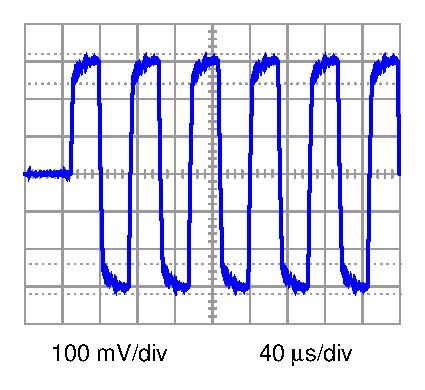
\includegraphics[width=15.5cm]{i01511x01.eps}$$

Undersøk følgende bølgeformer vist på et oscilloskop for FOUNDATION Fieldbus-signaler, og avgjør hvilken(e) feil som kan forårsake hver av dem. Pass på å forklare begrunnelsen bak hver diagnose!

\vskip 10pt

\centerline{\bf Eksempel \#1:} 

$$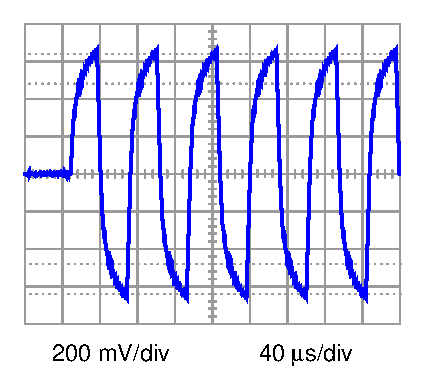
\includegraphics[width=15.5cm]{i01511x02.eps}$$

\vskip 10pt

\filbreak

\centerline{\bf Eksempel \#2:} 

$$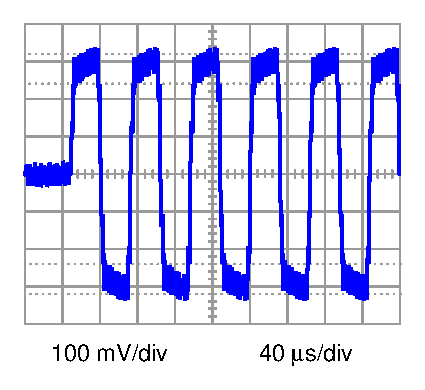
\includegraphics[width=15.5cm]{i01511x03.eps}$$

\vskip 20pt \vbox{\hrule \hbox{\strut \vrule{} {\bf Forslag til sokratisk diskusjon} \vrule} \hrule}

\begin{itemize}
\item{} I hvert av opptakene er datastrømmen som representeres av Fieldbus-signalet den samme. Identifiser bitene i denne datastrømmen, og forklar hvordan du kan vite sikkert hva de er.
\item{} Forklar hvordan vi kan avgjøre om hver flanke i bølgeformen er en ekte (klokket) databit, eller om noen av dem bare er overgangsflanker i klargjøringen av neste bit.
\item{} Tror du det ville være mulig å bruke et digitalt multimeter (DMM) i stedet for et oscilloskop og få den samme diagnostiske informasjonen? Med andre ord: er det nødvendig å se den faktiske {\it formen} på bølgeformen for å diagnostisere problemet i FF-segmentet?
\end{itemize}


\underbar{file i01511}
%(END_QUESTION)





%(BEGIN_ANSWER)

Datastrømmen er {\tt 101010101010}, basert på det vi vet om Manchester-koding generelt og FOUNDATION Fieldbus-signaler spesielt.

%(END_ANSWER)





%(BEGIN_NOTES)

Vi vet at datastrømmen er en alternerende sekvens av 1-ere og 0-er på grunn av bølgeformens frekvens: 15.625 kHz (perioden er 1.6 ruter multiplisert med 40 mikrosekunder per rute). Dette forteller oss at overgangene (stigende og fallende flanker) skjer så sakte som de kan i et FF-system. Med andre ord er hver overgang en ekte databit, ikke en ``klargjøring'' for å generere en gjentakende bit.

Hvis frekvensen var 31.25 kHz (maksimalt mulig i et FF H1-segment), ville vi vite at annenhver overgang var en ``klargjøring'', og at hver stigende flanke var en databit.

\vskip 10pt

Amplituden er altfor høy i eksempel 1 (1.36 volt P-P), noe som tyder på at én eller flere termineringsmotstander mangler i nettverket.

\vskip 10pt

Det er tydelig mye støy i eksempel 2 (omtrent 60 mV P-P).

\vfil \eject

\noindent
{\bf Oppsummeringsquiz:}

Identifiser en sannsynlig årsak til at et FOUNDATION Fieldbus H1-nettverkssignal har for stor signalamplitude (unormalt høy topp-til-topp-spenning):

\begin{itemize}
\item{} Feil kabeltype (A, B, C eller D)
\vskip 5pt 
\item{} For høy DC-forsyningsspenning
\vskip 5pt 
\item{} Kortslutning i segmentkabel
\vskip 5pt 
\item{} Jordfeil i segmentkabel
\vskip 5pt 
\item{} Manglende termineringsmotstand
\vskip 5pt 
\item{} For lang makrosyklus
\end{itemize}


%INDEX% Electronics review: oscilloscope usage
%INDEX% Fieldbus, FOUNDATION (H1): segment troubleshooting

%(END_NOTES)

